%! Author = Philipp Emmenegger
%! Date = 10/06/2021

\section{Declaring Types and Classes}
\subsection{Type Declarations}
\begin{itemize}
    \item New name for an existing type
    \item Can make other types easier to read
    \item Can have type parameters
    \item Can be nested
    \item Cannot be recursive
\end{itemize}
\begin{lstlisting}
type String = [Char]
-----------------------
type Pos = (Int, Int)
origin :: Pos
origin = (0, 0)

left :: Pos -> Pos
left (x,y) = (x-1, y)

-- Type parameter --
type Pair a = (a,a)
mult :: Pair Int -> Int
mult (m,n) ) m*n

-- Nested --
type Trans = Pos -> Pos
\end{lstlisting}

\subsection{Data Declarations}
\begin{itemize}
    \item Completely new type by specifying its values
    \item Values of new types can be used the same ways as built in types
    \item Constructors may also have parameters
    \item May also have type parameters
    \item Can be recursive
\end{itemize}
\begin{lstlisting}
data Bool = False | True
data Answer = Yes | No | Unknown

-- Parameter --
data Shape = Circle Float | Rect Float Float
square :: Float -> Shape
square n = Rect n n

-- Type parameters --
data Maybe a = Nothing | Just a

-- Recursive --
data Nat = Zero | Succ Nat
Succ (Succ (Succ Zero)) = 3
\end{lstlisting}

\subsection{Polymorphism}
\begin{enumerate}
    \item Ad-hoc Polymorphism: function with the same name denotes different implementations (function overloading / interfaces)
    \item Parametric Polymorphism: Code written to work with many possible types
    \item Subtype Polymorphism: one type can be substituted for another (subtype / supertype)
\end{enumerate}

\subsection{Type Classes}
\begin{itemize}
    \item Declared using class declarations
\end{itemize}
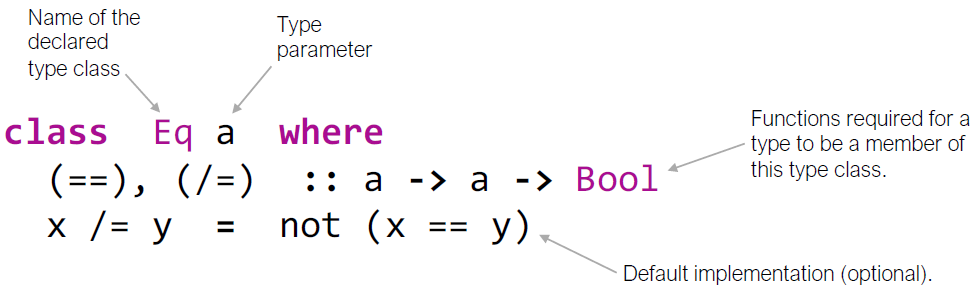
\includegraphics[width=0.7\linewidth]{img/class_declarations.png}